\section{Irregular orbits: Part 1}
% Most often, one does not know the fraction of irregular orbits for particular density model. A very useful technique for both determining whether an orbit is regular or irregular and classifying the type of orbit
% is the “surface of section” method. 
%This is described in detail in B\&T section 3.2.2.
% Adapt your ODE program to find the $x-\Dot{x}$ surface of section that
% is, have your program plot with points the the values of $x$ and $\Dot{x}$
% when $y = 0$ and $\Dot{y}> 0$.
% Use your ODE program to find a tube orbit and a box orbit in the
% potential given by B\&T equation 3-103 with $R_c = 0.14$, $q = 0.9$
% and $v_c = 1$. (See Figure 3-8 for inspiration).
% Now, plot the surface of section for these orbits. Note/discuss/explain
% the differences. [We will explore the surface of sections for irregular orbits in a later PS.]
The surface of section method is a very useful technique for both determining whether an orbit is regular or irregular and classifying the type of orbit.

A regular orbit is

A irregular orbit is

The possible types of orbits are

The logarithmic potential given by B\&T equation 3-103 is
\begin{equation}
    \Phi_L(x,y)=\frac{1}{2}v_0^2\log\left(R_c^2+x^2+\frac{y^2}{q^2}\right).
\end{equation}

The equations of motion for this system are:
\begin{align}
    a=-\nabla\Phi(x,y,)\\
    \ddot{x}=-\frac{v_o^2x}{R_c^2+x^2+\frac{y^2}{q^2}}\\
    \ddot{y}=-\frac{v_o^2x}{q^2\left(R_c^2+x^2+\frac{y^2}{q^2}\right)}
\end{align}

\begin{table}[]
    \centering
    \begin{tabular}{lrrrrr}
\toprule
{} &    x &    y &  $v_x$ &  $v_y$ &   Time \\
\midrule
Box Orbit   & 0.50 & 0.00 &   1.00 &   0.10 & 100.00 \\
Tube Orbit  & 0.00 & 0.20 &   1.00 &   0.00 & 100.00 \\
\bottomrule
\end{tabular}

    \caption{Caption}
    \label{tab:logIV}
\end{table}

Using $R_c=0.14$, $q=0.9$, $v_0=1$ and the initial conditions listed in Table \ref{tab:logIV}, we can integrate the orbits. Figure \ref{fig:logBox1} shows a box orbit and its surface of section on the plane when $y=0$.

\begin{figure*}
    \centering
    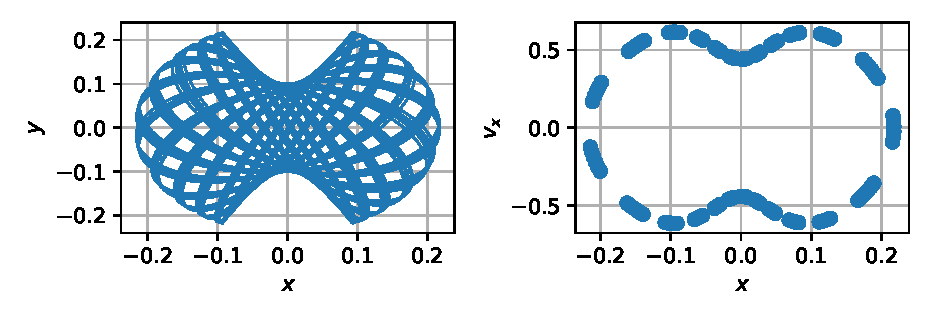
\includegraphics{CodeAndFigures/LogPotentialBoxOrbitPlot.pdf}
    \caption{Example of a box orbit using initial conditions listed in Table \ref{tab:logIV} and its surface of section on the plane $y=0$.}
    \label{fig:logBox1}
\end{figure*}

Figure \ref{fig:logBox2} shows a second box orbit and its surface of section on the plane when $y=0$. Note that instead of being confined in a rectangular area it is now in a eliptical area. 

\begin{figure*}
    \centering
    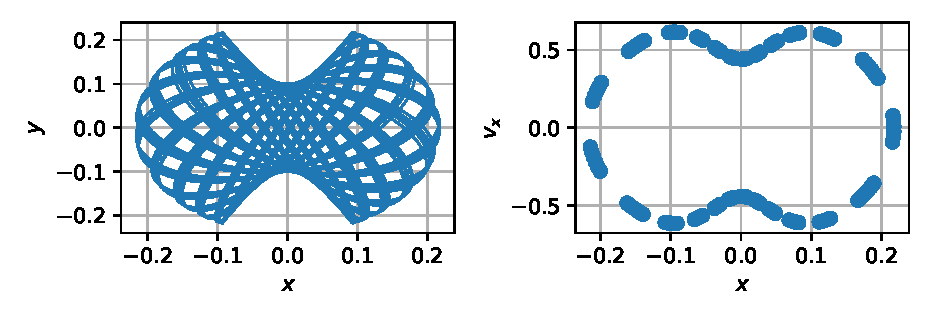
\includegraphics{CodeAndFigures/LogPotentialBoxOrbit2Plot.pdf}
    \caption{Second example of a box orbit using initial conditions listed in Table \ref{tab:logIV} and its surface of section on the plane $y=0$.}
    \label{fig:logBox2}
\end{figure*}

Figure \ref{fig:logTube} shows a tube orbit and its surface of section on the plane when $y=0$.

\begin{figure*}
    \centering
    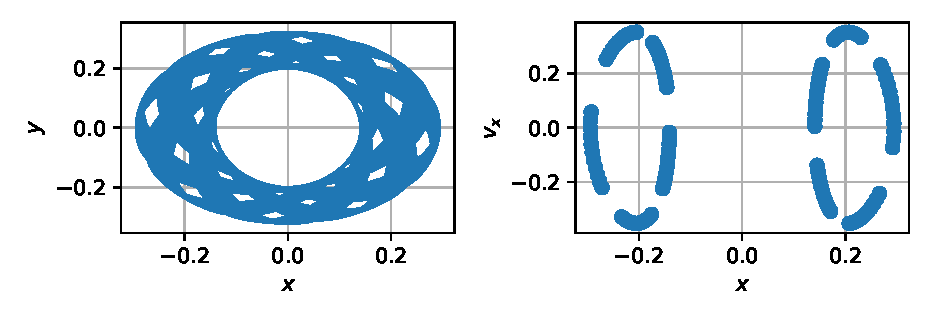
\includegraphics{CodeAndFigures/LogPotentialTubeOrbitPlot.pdf}
    \caption{Example of a tube orbit using initial conditions listed in Table \ref{tab:logIV} and its surface of section on the plane $y=0$ on a logarithmic potential.}
    \label{fig:logTube}
\end{figure*}



\clearpage